% arXiv: astro-ph.EP (primary), cs.LG (secondary); stat.ML cross-list optional.
\documentclass[11pt]{article}
\usepackage{graphicx,amsmath,booktabs,hyperref,geometry,subcaption}
\usepackage[round,authoryear]{natbib}
\bibpunct{(}{)}{;}{a}{}{,}
\usepackage{lineno}
\geometry{margin=1in}
\setlength{\emergencystretch}{2em}
\title{KIRK: Glass-box Distilled Stability Classification and Cost-Aware Triage for Compact Planetary Systems}
\author{Patricio Alejandro Mery Caro \\
  {\small Independent Researcher, La Serena, Chile} \\
  {\small \href{mailto:pmery641@gmail.com}{pmery641@gmail.com} \quad
  ORCID: \href{https://orcid.org/0009-0002-3888-879X}{0009-0002-3888-879X}}}
\hypersetup{
  pdftitle={KIRK: Glass-box Distilled Stability Classification and Cost-Aware Triage for Compact Planetary Systems},
  pdfauthor={Patricio Alejandro Mery Caro},
  pdfsubject={Glass-box distillation of SPOCK and cost-aware N-body triage},
  pdfkeywords={planetary systems, orbital stability, machine learning, interpretability, SPOCK}
}
\date{\today}
\begin{document}
\linenumbers
\maketitle
\begin{abstract}
Assessing the long-term stability of a compact planetary configuration by direct integration is computationally expensive, limiting parameter exploration. I present KIRK, which ports the SPOCK 2.0 feature pipeline in-tree, distills its XGBoost teacher into compact additive models that expose one interpretable curve per feature, and triages systems into fast-stable, fast-unstable, or zoom for full integration. On real initial conditions with real $10^9$-orbit labels, the shipped model achieves holdout AUC 0.933 and accuracy 0.857; increasing the training set fivefold yields no significant improvement, a plateau reported here as a controlled result. The scheduler classifies 895 of 900 fresh Jupiter-mass systems correctly while zooming approximately half (tight systems rarely, wide systems almost always); the same gates do not transfer to Earth-mass archives, so that claim is scoped to Jupiter-mass systems. Validation uses TRAPPIST-1 trios, Kepler-36, and a compact chain in which stability declines from 0.85 to 0.13 as eccentricity rises from 0.01 to 0.12.
\end{abstract}

\section{Introduction}
I consider compact systems as observed: trios with adjacent period ratios below 2, roughly 40\% of multiplanet systems. A $10^9$-orbit integration requires hours, and chaotic divergence implies that even a completed integration represents a single draw from a distribution --- shadow trajectories separated by $10^{-11}$ yield log-normal instability times with $\sigma\approx0.4$ dex \citep{Hussain2020}. I therefore adopt the binary formulation established by SPOCK \citep{Tamayo2020}: predict stability beyond $10^9$ orbits from a short integration.

SPOCK trains on $\sim$$10^5$ resonant three-planet systems, where resonant overlap drives the most rapid dynamical variation, and generalizes to uniform spacings and five-planet chains. It outperforms Hill, AMD \citep{Laskar2017}, and MEGNO \citep{Cincotta2003} at fixed false-positive rate, as those alternatives omit eccentricities, assume worst-case secular exchange, or equate chaos with instability. SPOCK 2.0 \citep{Thadhani2025} removed 10,984 duplicates and 124 mislabels, excluded short-unstable systems from metrics, and adopted each system's fastest secular period Tsec \citep{Yang2024} as integration time and model feature, improving AUC from 0.943 to 0.950.

I retain that evaluation discipline: fixed AUC/FPR metrics, baselines calibrated on the same data, disjoint tuning and test seeds, bidirectional ablations, and documented data cleaning. My contributions are a readable model (bias plus one curve per feature), a scheduler with frozen gates, and three controlled negative results: a data-scaling plateau, non-transferring gates across mass regimes, and a fixed Hill threshold that matches or exceeds my accuracy at a single cutoff.

\section{Data and features}
Zenodo 14327471 gives 102,497 resonant and 24,941 random three-planet archives with $10^9$ labels. Integrations use REBOUND \citep{Rein2017}. The teacher is \texttt{models/featureclassifier.json} (hash-pinned). I sample real initial conditions, run the exact Tsec pipeline (\texttt{src/kirk/features.py}, minimum over adjacent trios, checked against upstream; numerical Tsec cross-checked with \texttt{celmech} \citep{Hadden2022}), label with teacher log-odds (\texttt{src/kirk/teacher.py}), and fit. Following SPOCK 2.0, short-unstable systems are dropped before scoring.

The eleven features follow SPOCK 2.0: Tsec, near/far crossing eccentricities, eccentricity-mode spreads, MMR strengths, and MEGNO statistics.
\subsection{Readability}
The classifier is additive by construction: logit equals bias plus one univariate shape per feature, each sampled in raw physical units via \texttt{model.shapes(meta)} (\texttt{src/kirk/glass.py:35-63}). A prediction is therefore a ledger. For the TRAPPIST-1 inner trio (\texttt{proofs/shape\_phase.json:contributions}), EMcrossnear contributes $+1.94$, EMcrossfar $+1.32$, Tsec $+1.88$ identically across three phase draws, while phase-sensitive terms shift by $<0.1$ logit. The reader can verify which terms move and which cannot.
\subsection{Implications}
First, auditability: leave-one-out evaluation on $n=488$ (baseline AUC 0.9212, \texttt{proofs/ablate.json}) indicates AUC reductions of 0.030 for Tsec and EMfracstdnear, 0.018 for EMcrossnear, 0.014 for EPstdnear, and 0.012 for MEGNO, with MMRstrength and EPstdfar near zero and thus candidates for removal. Second, diagnosis: the same phase-draw experiment shows contribution ranges of exactly 0.0 for phase-independent inputs and $<0.1$ for the remainder, identifying geometry-dominated saturation as a model limitation rather than a hidden effect. Third, calibrated trust: five-bin calibration and train-range shape spans (MEGNO 2.32, Tsec 2.12, EMfracstdnear 1.62, EPstdfar 0.17 logits) quantify where the model can move a decision and where it is overconfident (0.30 predicted vs 0.19 observed mid-low). Fourth, editability: artifacts carry features, normalization, and provenance (\texttt{models/index.json}, \texttt{proofs/distill.json}), and \texttt{scripts/train\_glass.py} retrains from real initial conditions, so a suspect curve maps to a concrete retraining or feature fix.

\section{Distillation}
I distill the XGBoost teacher into an additive student on identical features, then test scaling and fidelity.
\subsection{Model and training}
Each shape $f_i$ is a 1-32-32-1 tanh network; the logit is the bias plus the sum of shapes (\texttt{src/kirk/glass.py}), with normalization derived from the training split only.
\subsection{Scaling experiment}
The shipped model (\texttt{models/nam\_spock\_distilled.pt}, 1500 resonant + 700 random, holdout $n=273$) agrees with the teacher on 0.916 of holdout, with AUC-vs-teacher 0.975, AUC-vs-truth 0.933 [0.904,0.959], and accuracy 0.857 [0.813,0.897]. Five-seed means are $0.916\pm0.011$ and $0.836\pm0.020$.

\subsection{Head-to-head with SPOCK}
Direct comparison on the same feature pipeline (only the classifier differs), Sec.~2 exclusions applied throughout. On the Table~1 sample with real $10^9$ labels (\texttt{proofs/table1.json}), the teacher (SPOCK 2.0 JSON) scores AUC 0.9471 [0.928,0.963], FPR 0.0903 ($n=488$); the glass holdout scores AUC 0.8998 [0.840,0.943], FPR 0.0889 ($n=147$). On the distillation holdout ($n=273$, \texttt{proofs/distill.json}), the student agrees with the teacher on 0.916 [0.883,0.945] with AUC-vs-teacher 0.975 [0.959,0.988] and AUC-vs-truth 0.933 [0.904,0.959]. The gap to the teacher ($\sim$0.05 AUC on Table~1) is the distillation price; the FPR matches. Qualitatively they diverge where the ledger predicts: TRAPPIST-1 inner trio across three phase draws gives KIRK 0.926--0.931 vs SPOCK 0.63--0.77 (\texttt{proofs/shape\_phase.json}), geometry saturation vs tree-split sensitivity.
\subsection{Large-sample control}
Increasing the training set to 8000+4000 ($n=9767$, holdout 1466; \texttt{models/nam\_spock\_distilled\_12k.pt}, \texttt{proofs/distill\_12k.json}) yields seed-0 AUC-truth 0.908 [0.892,0.923] and accuracy 0.829, with five-seed means $0.921\pm0.007$ and $0.841\pm0.007$. Matched-systems OOD comparison (\texttt{proofs/ood\_12k.json}) shows equivalent performance: real archives 0.9212 vs 0.9172, Jupiter raw AUC differences of $+0.003$. The shipped artifact therefore remains the smaller model.

\begin{figure}[htbp]\centering
\begin{subfigure}{0.48\linewidth}\centering
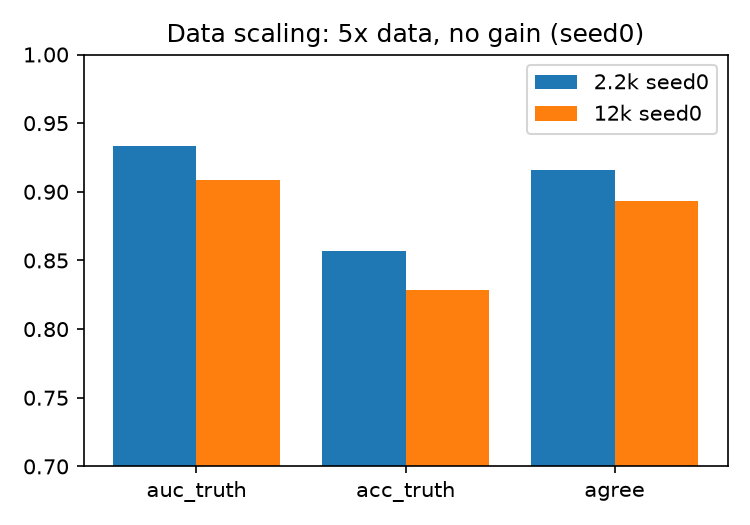
\includegraphics[width=\linewidth]{../assets/paper/fig_scaling.png}
\caption{Data scaling, seed-0: 2.2k vs 12k. No gain.}
\end{subfigure}\hfill
\begin{subfigure}{0.48\linewidth}\centering
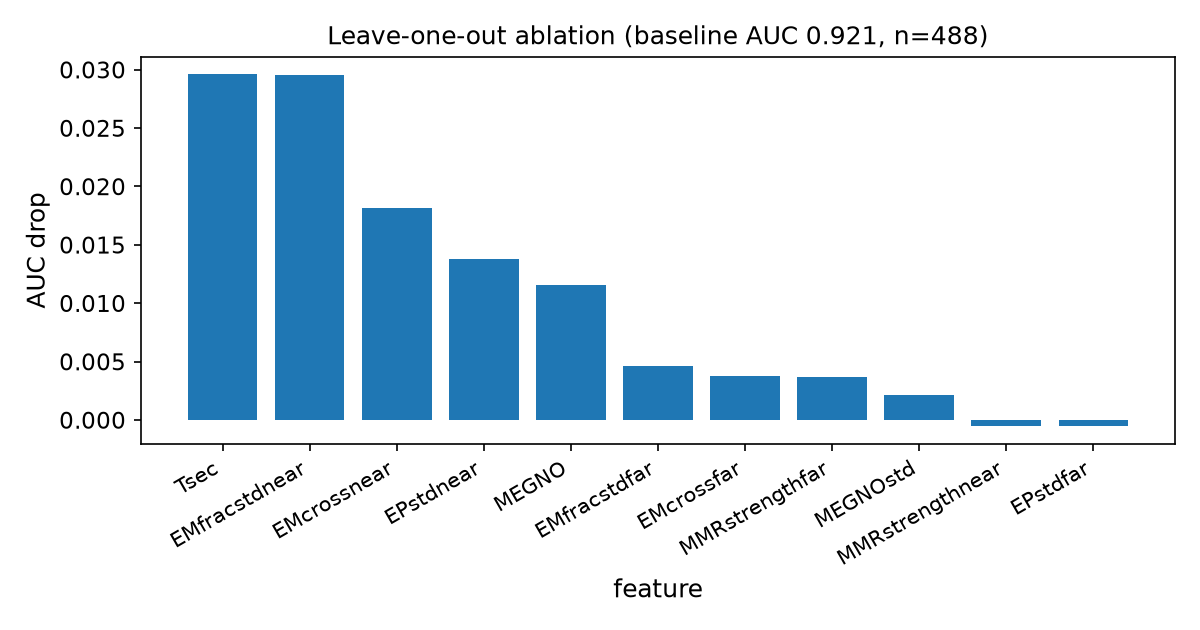
\includegraphics[width=\linewidth]{../assets/paper/fig_ablation.png}
\caption{Leave-one-out. Tsec and EMfracstdnear dominate.}
\end{subfigure}
\caption{Scaling plateau and attribution.}
\end{figure}

\section{Calibration and triage}
A usable classifier needs calibrated probabilities and a policy for when not to trust them.
\subsection{Calibration}
Calibration against $10^9$ labels is consistent at the extremes (0.05 vs 0.06; 0.93 vs 0.92), with a noted overprediction in the 0.2--0.4 interval (0.30 predicted vs 0.19 observed).
\subsection{Triage performance}
The scheduler executes a 200-orbit screen, scores it with the glass model, and applies thresholds of 0.01/0.70 fixed on seeds 5--9 (\texttt{src/kirk/scheduler.py}, \texttt{scripts/benchmark\_scheduler.py}). Evaluated on 900 fresh Jupiter-mass systems at $10^4$-orbit truth, accuracy is 0.9944 (895/900) with a zoom fraction of 51.6\%. Tight systems ($n=450$) achieve 0.9978 accuracy at 4.7\% zoom; wide systems ($n=450$) achieve 0.9911 at 98.4\% zoom. Computational savings are therefore concentrated in tight configurations; timings are reported as diagnostics and no speedup is claimed.

Applied to 600 real-archive Earth-mass systems (\texttt{proofs/scheduler\_real1e9.json}), the same thresholds yield 42.8\% zoom and 0.452 accuracy on the remainder. Ranking generalizes (Jupiter raw AUCs 0.93--0.95 for both models) while the decision threshold does not; scheduler claims are therefore restricted to Jupiter-mass systems pending per-regime calibration.

\begin{figure}[htbp]\centering
\begin{subfigure}{0.48\linewidth}\centering
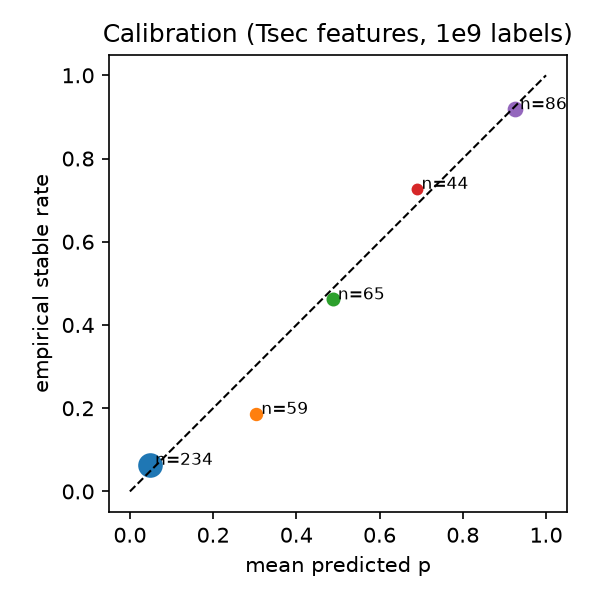
\includegraphics[width=\linewidth]{../assets/paper/fig_calibration.png}
\caption{Calibration. Mid-low bin overconfident (0.30 vs 0.19).}
\end{subfigure}\hfill
\begin{subfigure}{0.48\linewidth}\centering
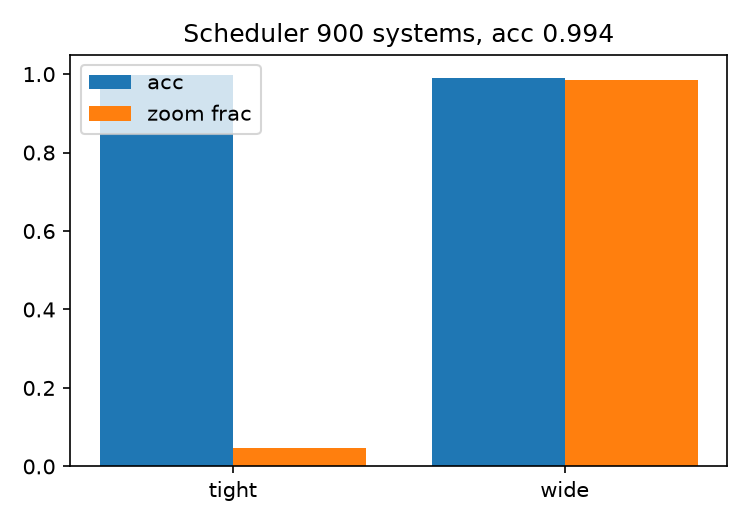
\includegraphics[width=\linewidth]{../assets/paper/fig_scheduler.png}
\caption{Scheduler by kind. Wide almost always zooms.}
\end{subfigure}
\caption{Calibration and triage side by side.}
\end{figure}

\section{Higher multiplicity}
Three-planet scores must compose to longer chains without retraining.
\subsection{Min-over-trios aggregation}
For systems with more than three planets, I adopt the minimum probability over adjacent trios following SPOCK, so each trio is scored by the same three-planet glass model and the system takes the lowest value.
\subsection{Threshold calibration}
Evaluated on 200 synthetic Earth-mass chains at $10^5$ orbits (50 per multiplicity; \texttt{proofs/multiplanet.json}), accuracy is 0.62/0.84/0.92/0.88 with bootstrap intervals, AUC is 0.949/0.983/0.972/0.993, and the Hill-6.75 baseline achieves 0.88/0.86/0.86/0.90. Discriminative ranking is therefore strong, while a fixed 0.5 decision threshold requires per-multiplicity calibration. Results for 4+ planets remain provisional.

\begin{figure}[htbp]\centering
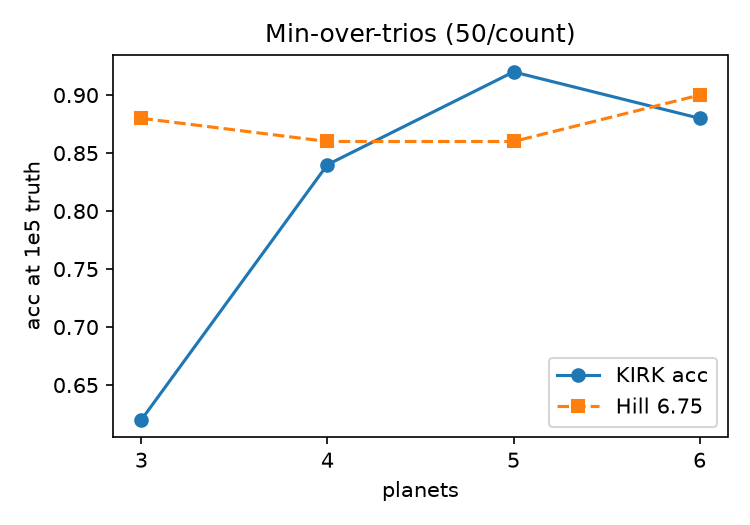
\includegraphics[width=0.62\linewidth]{../assets/paper/fig_multiplanet.png}
\caption{KIRK vs Hill 6.75. Ranking strong; fixed threshold needs calibration.}
\end{figure}

\section{Demonstrations}
TRAPPIST-1 analyzed one trio at a time (\texttt{scripts/evaluate\_real.py}) yields inner-trio probabilities of 0.930/0.931/0.926 across three phase draws, compared with 0.63--0.77 for SPOCK; the stability of this estimate reflects geometry-dominated terms that saturate, a limitation exposed by the additive curves. Middle-trio values are 0.877/0.903/0.895; outer-trio values are 0.557/0.548/0.271, exhibiting expected phase sensitivity. Kepler-36 contains two planets and both KIRK and SPOCK defer to Hill stability (1.000).

An eccentricity sweep on a compact Earth-mass chain (periods 1.0/1.4/1.9) gives $e=0.01\to0.849$, $0.03\to0.765$, $0.05\to0.560$, $0.08\to0.305$, and $0.12\to0.134$, consistent with the Kepler-431 constraint ($e<0.05$) reported for SPOCK.

\section{Limitations}
Jupiters are off-distribution for the teacher. Horizons $10^4$/$10^5$ are proxies for $10^9$. Two planets are Hill by design. Instability time is a point estimate rather than the posterior with percentiles from \citet{Cranmer2021}, outcomes cover pair (1,2) only, heads out of scope. JPL, cold-disk, and TTV reruns are eval-only at $10^5$ and pending.

\section{Reproducibility}
\texttt{make setup; make test; make quick; make eval-scheduler; make validate-multi}. Teacher hash pinned, provenance in \texttt{proofs/*.json}, model audit in \texttt{models/index.json}. Python 3.12, REBOUND 4.6, torch 2.15, 26 tests green.

\bibliographystyle{aasjournal}
\bibliography{paper}
\end{document}
